% !TEX encoding = UTF-8 Unicode
\documentclass{standalone}
% \usepackage{pgfplots}
% \pgfplotsset{compat=1.11}
\usepackage{amsmath}
\usepackage{amsfonts}
\renewcommand{\familydefault}{\sfdefault}
% \usepackage[version=0.96]{pgf}
\usepackage{tikz}
% \usetikzlibrary{arrows,shapes,automata,backgrounds,petri,positioning}
% \usetikzlibrary{decorations.pathmorphing}
% \usetikzlibrary{decorations.shapes}
% \usetikzlibrary{decorations.text}
% \usetikzlibrary{decorations.fractals}
% \usetikzlibrary{decorations.footprints}
% \usetikzlibrary{shadows}
% \usetikzlibrary{calc}
% \usetikzlibrary{spy}

% \pgfplotsset{compat=1.11}
\usepackage[utf8]{inputenc}
% \usepackage[vietnam]{babel}

\def\d{.6}
% \def\p{5.1}
\def\q{-.6}
% \def\sc{25}

\newcommand{\nn}[4]{
    \begin{scope}[xshift = #1*\d cm, yshift = #2*\q cm]
        
    \node at (0, 0) [anchor = east, draw, inner sep = 0, fill = #3!20, minimum height = .6cm, minimum width = .6cm] {#4};
    \end{scope}
}

\newcommand{\nnn}[4]{
    \begin{scope}[xshift = #1*\d cm, yshift = #2*\q cm]
        
    \node at (0, 0) [anchor = east, align = left,  draw, inner sep = 0, fill = #3!30, minimum height = .6cm, minimum width = .6cm] {#4};
    \end{scope}
}



\begin{document}
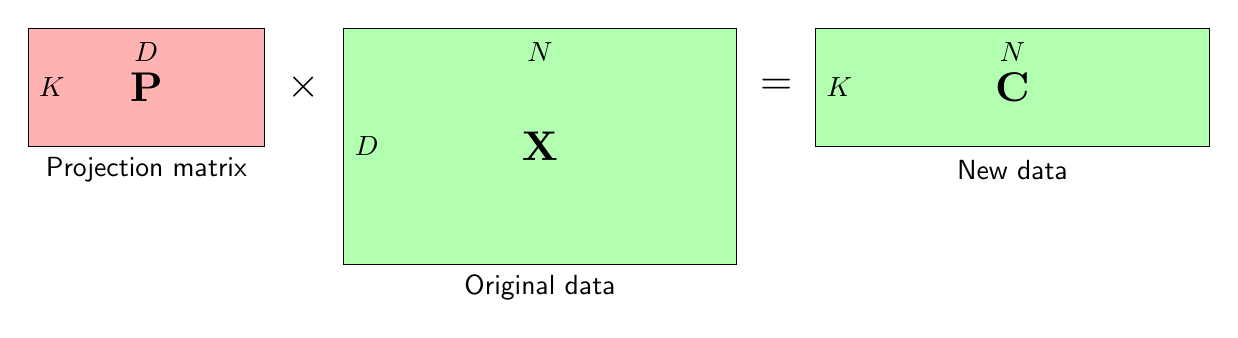
\begin{tikzpicture}
    \begin{scope}
        \draw [fill = green!30] (0, 0) rectangle (5, 3);
        \node [scale = 1.5] at (2.5, 1.5) {$\mathbf{X}$};
        \node at (2.5, -0.3) {Original data};
        \node at (2.5, 2.7) {$N$};
        \node at (.3, 1.5) {$D$};
        \node [scale = 1.5] at (5.5, 2.25) {$=$};
    \end{scope}

    \begin{scope}[xshift = -4cm]
        \draw [fill = red!30] (0, 1.5) rectangle (3, 3);
        \node [scale = 1.5] at (1.5, 2.25) {$\mathbf{P}$};
        \node at (1.5, 1.2) {Projection matrix};
        \node at (1.5, 2.7) {$D$};
        \node at (.3, 2.25) {$K$};
        \node [scale = 1.5] at (3.5, 2.25) {$\times$};
    \end{scope}

    \begin{scope}[xshift = 6cm, yshift = 1.5cm]
        \draw [fill = green!30] (0, 0) rectangle (5, 1.5);
        \node [scale = 1.5] at (2.5, .75) {$\mathbf{C}$};
        \node at (2.5, -0.3) {New data};
        \node at (2.5, 1.2) {$N$};
        \node at (.3, .75) {$K$};
        % \node [scale = 1.5] at (5.5, .75) {$=$};
    \end{scope}

    % \begin{scope}[xshift = 6cm]
    %     \draw [fill = red!30] (0, 0) rectangle (1.6, 3);
    %     \node [scale = 1.5] at (.8, 1.5) {$\mathbf{X}$};
    %     \node at (.3, 1.5) {$M$};
    %     \node at (.8, 2.7) {$K$};
    %     \node [scale = 1.5] at (1.9, 2) {$\times$};
    %     \node at (.8, -0.3) {Item features};
    %     \node at (.8, 3.7) [scale = 1.5] {$\mathbf{Y} \approx \hat{\mathbf{Y}} = \mathbf{XW}$};
    % \end{scope}

    % \begin{scope}[xshift = 8.2cm]
    %     \draw [fill = cyan!30] (0, 3) rectangle (5, 1.4);
    %     \node [scale = 1.5] at (2.5, 2.2) {$\mathbf{W}$};
    %     \node at (0.3, 2.2) {$K$};
    %     \node at (2.5, 2.7) {$N$};
    %     \node at (2.5, 1.1) {User features};
    % \end{scope}

\end{tikzpicture}
\end{document}